\justifying
\NSFCBodyText

\subsubsection{年度研究计划}

本项目执行期为 2027 年 1 月至 2030 年 12 月，共 4 年。各年度任务安排如下，其中月份划分与工作量分配为计划安排\textbf{【暂定】}，将根据实际进展调整。 四年任务安排与 H1 检验节点见图~\ref{fig:timeline}。

% F10: F10_年度研究计划.png
\begin{figure}[!htbp]
    \centering
    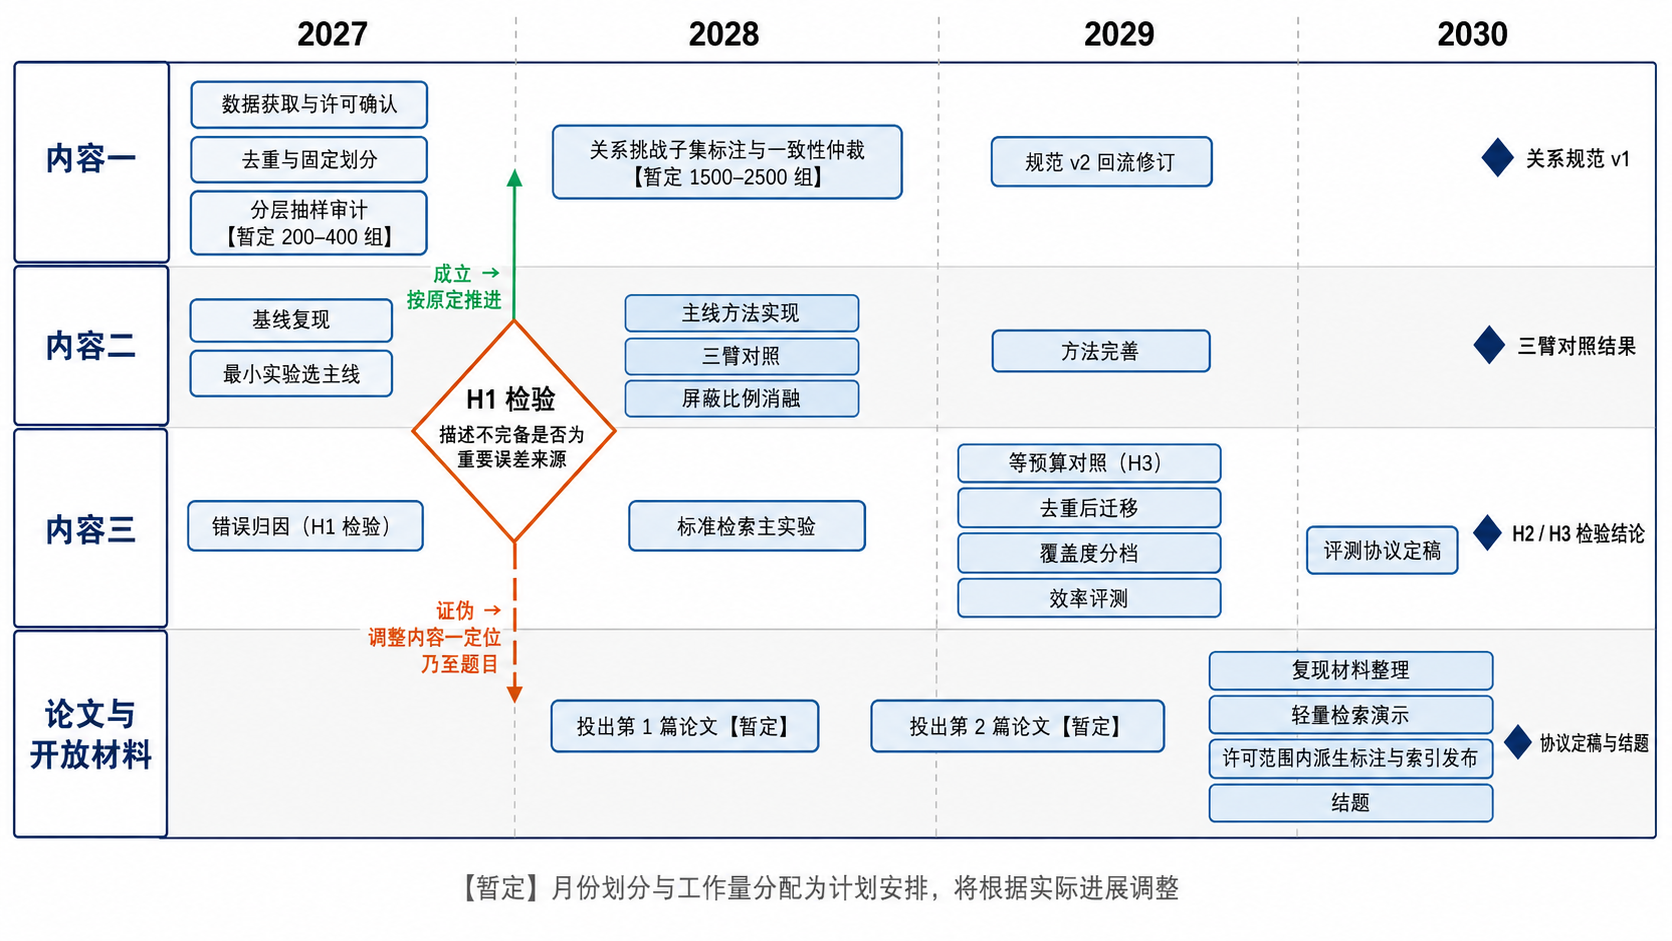
\includegraphics[width=\linewidth]{figures/F10_年度研究计划.png}
    \caption{年度研究计划与里程碑。执行期为 2027.01--2030.12，H1 检验前置于第一年；阶段目标以本节逐年说明为准。}
    \label{fig:timeline}
\end{figure}


\subsubsubsection{第一年（2027.01--2027.12）：数据基础与假说检验}

本年度的核心任务是\textbf{检验假说 H1}，即确认"描述不完备"是否确实构成检索失效的重要成因。这决定后续三年的研究定位，因此安排在最前。

具体工作包括：完成数据获取、完整性核对与许可确认，对原图、近重复影像与同源切片去重并建立固定划分；对每个基准分层抽样\textbf{【暂定 200--400 组】}影像及其全部配对描述开展语义审计；复现 CLIP\cite{radford2021clip}、RemoteCLIP\cite{liu2024remoteclip} 及参数高效适配\cite{yuan2023peft}对照基线；在基线错误上开展人工核验的错误归因，区分"描述未覆盖""关系冲突""细粒度语义不足""同类场景近似"等成因；建立实体关系词表与三态判定规范初版；开展最小方法实验，从三条候选实现路线中选定主线。

\textbf{阶段目标}：数据审计报告、可复现基线配置与结果、H1 检验结论（含证伪时的方案调整决定）、关系词表与判定规范 v1、主线路线选定。

\subsubsubsection{第二年（2028.01--2028.12）：关系挑战集与方法实现}

具体工作包括：完成关系挑战子集\textbf{【暂定 1500--2500 组】}的双人独立标注、一致性评估与仲裁，剔除一致性不达标的关系类型；实现内容二主线方法并完成三臂对照，严格对齐骨干、训练预算与数据划分；在 RSITMD、RSICD 上完成标准检索主实验；开展初步消融，分析屏蔽比例与训练稳定性的关系。

\textbf{阶段目标}：关系挑战子集 v1 与一致性报告、核心方法与训练推理代码、三臂对照结果、投出第 1 篇论文\textbf{【暂定】}。

\subsubsubsection{第三年（2029.01--2029.12）：可归因性验证与方法完善}

具体工作包括：完成等参数量、等训练步数对照实验以检验 H3；开展去重后的跨数据集迁移测试，并将同域比较、迁移测试与数据独立测试分别报告；完成覆盖度分档稳健性评测；根据评测暴露的失效模式回流修订关系词表与判定规范；完成效率评测。

\textbf{阶段目标}：完整分层评测结果、H2 与 H3 检验结论、关系规范 v2、投出第 2 篇论文\textbf{【暂定】}。

\subsubsubsection{第四年（2030.01--2030.12）：独立验证、开放材料与结题}

具体工作包括：完成独立验证与补充实验，处理论文返修；整理复现材料（环境说明、固定划分、模型来源、随机种子、运行说明与实验日志）；开发轻量检索演示；在数据许可允许范围内发布派生标注或数据索引与构建脚本；完成评测协议定稿与项目总结。

\textbf{阶段目标}：评测协议定稿、开源代码与复现材料、轻量演示系统、结题报告。

\subsubsection{预期研究结果}

\subsubsubsection{学术成果}

在国内外高水平期刊或会议上发表学术论文\textbf{【暂定 4--6 篇】}，其中围绕关系证据建模、未知态屏蔽的匹配方法与分层评测协议各形成代表性成果。论文均按基金委要求标注资助信息。此处数量为计划口径\textbf{【暂定】}，最终以申请人可承担的范围为准，不作超出实际能力的承诺。

\subsubsubsection{方法与技术成果}

形成面向不完备描述的地理实体关系证据表示方法 1 套，包括实体关系词表、证据字段规范与三态判定规则；形成仅约束可核验关系、屏蔽未知态的跨模态匹配方法 1 套，含完整的三臂对照与消融证据。

\subsubsubsection{数据与工具成果}

形成经人工核验的关系挑战评测子集\textbf{【暂定 1500--2500 组】}与配套标注规范；形成可复现的算法代码 1 套，包含运行环境、固定数据划分、模型来源、随机种子、运行说明与实验日志；形成分层评测协议 1 套。受第三方数据许可限制，原始影像不作再分发；数据成果优先以索引、处理脚本、版本说明与获准发布的派生标注形式交付。

\subsubsubsection{人才培养}

培养研究生\textbf{【暂定 3--5 名】}，使其在跨模态检索、遥感图文理解与实验设计方面获得系统训练。

\subsubsubsection{关于成果表述的说明}

本项目\textbf{不预设任何量化性能提升指标}。截至申请时，本项目尚未完成数据下载核验与基线复现，因此任何形如"mR 提升若干百分点""关系判别准确率达到某一水平"的承诺都缺乏依据。相关指标将在第一年完成基线复现与错误归因后确定，并在中期检查时明确报告。若假说 H1 被证伪，本项目将如实报告负结果并调整研究定位，相应的预期成果口径同步修订。
